\chapter{Final report}

\section{Introduction}
To better explain the results of later chapters, quaternions and biquaternions are first introduced, along with their kinematic interpretations.
%% Biquaternions and biquaterionic polynomials



\subsection{Quaternions}
The algebra of quaternions -- usually denoted as $\mathbb{H}$ -- is homomorphic to the 3 dimensional special orthogonal group(SO(3)), which is the group representing rotations in 3D space. A general quaternion $h$ can be written as follows:
\begin{equation}
    h = h_0 + h_1i +h_2j + h_3k
\end{equation}
The 3 unit versors $i$,  $j$, $k$ are not commutative, and subject to the following equations:
\begin{equation}
       i^{2} = -1,\;
       j^{2} = -1,\;
       k^{2} = -1,\;
       ijk = -1
\end{equation}
A quaternion with its scalar par $h_0$ equal to zero is called a purely vectorial quaternion, the set of which is denoted as $\mathcal{H}$.  The conjugate of a quaternion is defined as:
\begin{equation}
    \bar{h} = h_0 - h_1i - h_2j - h_3k
\end{equation}
The conjugate can be used to define the square of the norm of a quaternion:
\begin{equation}
    h\bar{h} = \bar{h}h = h_0^{2} + h_1^{2}+h_2^{2} + h_3^{2} \in \mathbb{R}
\end{equation}
If $h \in \mathcal{H}$, then $h + \bar{h} = 0$.
\clearpage
\subsubsection{SO(3)}
Given $v \in \mathcal{H}$, a quaternion $p \in \mathbb{H}$ can be used to rotate it around the origin by the following map:
\begin{equation}
    v' = \frac{pv\bar{p}}{p\bar{p}}
\end{equation}
In particular, if $p$ is a unit quaternion with $p\bar{p} = 1$ we have:

\begin{equation}
    v' = pv\bar{p}
\end{equation}
This is sometimes affectionately referred to as the \textbf{sandwich product}.
\\
To understand how a sandwich product of a quaternion $p$ rotates $v$, it helps to observe, that every unit quaternion can be written as:
\begin{equation}
    p = \cos{(\frac{\theta}{2})} + \sin{(\frac{\theta}{2})}u
\end{equation}
where $u\bar{u} = 1$ and  $u\in \mathcal{H}$. Then the sandwich product represents rotation of $v$ around the axis $u$ by the angle $\theta$.
To convince ourselves of this, we can first see that a rotation of $u$ around $u$ leads to the identity transformation, and investigate the behaviour of unit versors.\\
\subsubsection{Rotation of a versor lying on the rotation axis}
\begin{equation}
    \begin{aligned}
        u'&=pv\bar{p}&\mbox{}\\[1.25ex]
        u'&=(\cos{(\frac{\theta}{2})}+\sin{(\frac{\theta}{2})u})u(\cos{(\frac{\theta}{2})}-\sin{(\frac{\theta}{2})u})&\mbox{}\\[1.25ex]
        u'&=(\cos{(\frac{\theta}{2})}+\sin{(\frac{\theta}{2})u})(\cos{(\frac{\theta}{2})}u+\sin{(\frac{\theta}{2})})&\mbox{}\\[1.25ex]
        u'&=(\cos{(\frac{\theta}{2})}^{2} + \sin{(\frac{\theta}{2})}^{2})u&\mbox{}\\[1.25ex]
        u'&=u&\mbox{}\\[1.25ex]
    \end{aligned}
\end{equation}
\subsubsection{Rotation of a basis versor around another basis versor}
Let $p = \cos{(\frac{\theta}{2})} + \sin{(\frac{\theta}{2})}k$, then if we calculate the sandwich products $pi\bar{p}$ or  $pj\bar{p}$ we should expect results similar to ones well known from linear algebra:\\

\noindent\begin{minipage}{.5\linewidth}
    \begin{equation}
        \begin{bmatrix}
            \cos{(\theta)} \\
            \sin{(\theta)} \\
            0
        \end{bmatrix} = \begin{bmatrix}
        \cos{(\theta)} & -\sin{(\theta)} & 0\\
        \sin{(\theta)} & \cos{(\theta)} & 0 \\
        0 & 0 & 1
        \end{bmatrix}
        \begin{bmatrix}
            1  \\ 0 \\ 0
        \end{bmatrix}
    \end{equation}
\end{minipage}
\begin{minipage}{.5\linewidth}
    \begin{equation}
             \begin{bmatrix}
            -\sin{(\theta)} \\
            \cos{(\theta)} \\
            0
        \end{bmatrix} = \begin{bmatrix}
        \cos{(\theta)} & -\sin{(\theta)} & 0\\
        \sin{(\theta)} & \cos{(\theta)} & 0\\
        0 & 0 & 1
        \end{bmatrix}
        \begin{bmatrix}
            0  \\ 1 \\ 0
        \end{bmatrix}
    \end{equation}
\end{minipage}
And in fact:
\begin{equation}
    \begin{aligned}
         u'&=pi\bar{p}&\mbox{}\\[1.25ex]
        u'&=(\cos{(\frac{\theta}{2})}+\sin{(\frac{\theta}{2})k})i(\cos{(\frac{\theta}{2})}-\sin{(\frac{\theta}{2})k})&\mbox{}\\[1.25ex]
        u'&=(\cos{(\frac{\theta}{2})}+\sin{(\frac{\theta}{2})k})(\cos{(\frac{\theta}{2})}i+\sin{(\frac{\theta}{2})}j)&\mbox{}\\[1.25ex]
        u'&=(\cos{(\frac{\theta}{2})}^{2}-\sin{(\frac{\theta}{2})}^{2})i + 2\sin{(\frac{\theta}{2})}\cos{(\frac{\theta}{2})}j&\mbox{}\\[1.25ex]
        u'&=\cos{(\theta)}i + \sin{(\theta})j&\mbox{}\\[1.25ex]

    \end{aligned}
\end{equation}
A result in complete agreement with one obtained by the use of rotation matrices

\clearpage

\subsubsection{T(3)}

Since we already associate the 3 basis versors with the 3 standard axes of a Cartesian space, it seems natural to use quaternions to represent translations. It is in fact trivial to do, a translation is simply the addition of one purely vectorial quaternion to another:
\begin{equation}
    v' = v + u
\end{equation}
where $v,u\in \mathcal{H}$.
\subsubsection{SE(3)}
The special Euclidean group(SE(3)), which represents rigid body motions in 3D space, is composed of 2 subgroups. Those being the special orthogonal group SO(3), and the translational group in 3D T(3). Given these 2, one can construct SE(3) as the semi-direct product of them as such:
\begin{equation}
    SE(3) = SO(3)\ltimes T(3)
\end{equation}
With this construction, elements of SE(3) are given by a tuple  $(r,t)$, and a product of 2 of its elements is given as follows:
 \begin{equation}
     \label{semidirect}
     (r_2,t_2)(r_1,t_1) = (r_2r_1,r_2t_1\bar{r}_2+t_2)
\end{equation}
With $r_1,r_2\in SO(3)$, and $t_1,t_2 \in T(3)$\\
This formula should be familiar to anyone who ever multiplied 2 DHT matrices together.\\
In general then, a pair of quaternions is enough to represent the motion of rigid bodies. A problem however with this formulation is that it requires pairs of quaternions, which makes it mathematically unwieldy. This leads to the idea of enclosing both of these pairs in a single algebra.
\subsection{Biquaternions}
The way the above issue can be solved when using orthogonal matrices to represent rotation, is to embed SE(3) in SO(4). This may sound complicated, but this is in fact the most common way to represent elements of SE(3). An example would be the block matrix:
\begin{equation}
    A_i = \begin{bmatrix}
        R & T   \\
        \mathbb{0} & 1
    \end{bmatrix}
\end{equation}
Again, this should be familiar to anyone who knows anything about robot kinematics. If we multiply 2 such matrices together we will obtain:
\begin{equation}
    A_1A_2 =  \begin{bmatrix}
        R_1 & T_1   \\
        \mathbb{0} & 1
    \end{bmatrix} 
 \begin{bmatrix}
        R_2 & T_2   \\
        \mathbb{0} & 1
    \end{bmatrix} 
 \begin{bmatrix}
        R_1R_2 & R_2T_1 + T_2\\
        \mathbb{0} & 1
    \end{bmatrix}
\end{equation}
Which looks exactly like the semi-direct product presented before \ref{semidirect}. Do tho this with quaternions however, we have to utilise a different method. A way to do this, is to introduce a new type of coefficient for 
regular quaternions. Instead of using real numbers $h_i \in \mathbb{R}$ as coefficients, one can introduce dual number coefficients $h_i \in \mathbb{D}$ $h_i = p_i + \varepsilon q_i$, where  $\varepsilon^{2} = 0$. By using these dual coefficients, we create a new algebra called the dual quaternions(sometimes also known as bi quaternions) which we will denote as $\mathbb{DH}$. An element $h \in \mathbb{DH}$ can also be written as 
 \begin{equation}
    h = p + \varepsilon q
\end{equation}
Where $p,q \in \mathbb{H}$. 
A necessary condition for a biquaternion to describe an element of SE(3) is that it lies in the Study quadric\cite{Heged_s_2013}. This condition for a biquaternion can be alternatively stated that it needs to have a real non-zero norm. A norm of a biquaternion is defined in terms of its conjugate as follows:
\begin{equation}
    \begin{aligned}
        h\bar{h}=(p+\varepsilon q)\bar{(p+\varepsilon q)}\\
        h\bar{h}=(p+\varepsilon q)(\bar{p}+\varepsilon \bar{q})\\
        h\bar{h}=p\bar{p} + \varepsilon (p\bar{q} + q\bar{p}) 
    \end{aligned}
\end{equation}
For the above to be a real number, the dual part needs to be zero, e.g. $  (p\bar{q} + q\bar{p}) = 0$. The rotation can be extracted by just taking the primal part p of the biquaternion. Its action upon elements of SE(3) is defined the same as for regular quaternions. The position of a point in space - represented as $x = 1+\varepsilon v$, where v is a vectorial quaternion - is given by the map\cite{Siegele_2021}:
\begin{equation}
     x \rightarrow \frac{(p - \epsilon q)x(\bar{p}+\epsilon \bar{q})}{p\bar{p}}
\end{equation}
Which can be rewritten:
\begin{equation}
    \label{act}
    \begin{aligned}
        \frac{(p - \epsilon q)x(\bar{p}+\epsilon \bar{q})}{p\bar{p}}&=\frac{px\bar{p} + \epsilon(px\bar{q} - qx\bar{p})}{p\bar{p}}&\\[1.25ex]
        \frac{px\bar{p} + \epsilon(px\bar{q} - qx\bar{p})}{p\bar{p}}&= 1+\epsilon\frac{pv\bar{p} + p\bar{q} - q\bar{p}}{p\bar{p}}&\\[1.25ex]
        1+\epsilon\frac{pv\bar{p} + p\bar{q} - q\bar{p}}{p\bar{p}}&= 1 + \epsilon \frac{pv\bar{p} + 2p\bar{q}}{p\bar{p}}&\\[1.25ex]
    \end{aligned}
\end{equation}

Note that the map does not require the biquaternion to be of unit norm. In fact, the mapped point remains the same no matter what real number we multiply the polynomial by. By noticing this, we can treat the space of rigid body motions as a projective space, allowing for the use of polynomials to represent trajectories in it. The simplest such motions are translations along a line, and rotation around a point. Both can be described using linear biquaterionic polynomials.

\subsubsection{Elementary motions}
A linear biquaterionic polynomial can represent either a translation, or a rotation. 
A general formula for a linear univariate biquaterionic polynomial parametrising a rigid body motion is the following:
\begin{equation}
    F = 1+th,\; h \in \mathbb{DH}
\end{equation}
To represent a motion in SE(3), its norm polynomial has to be real:
\begin{equation}
    F\bar{F} = 1+(h+\bar{h})t+h\bar{h}t^{2} \in \mathbb{R}[t]
\end{equation}
Since the parameter t is always real, this translates to:
\begin{equation}
    \begin{cases}
        h\bar{h} \in \mathbb{R}\\
        h+\bar{h} \in \mathbb{R}
    \end{cases}
\end{equation}
Since $h = p + \epsilon q,\; p,q \in \mathbb{H}$, this is equivalent to saying that $h$ itself has to satisfy the Study condition -- and so represent an element of SE(3) -- and has to have purely vectorial dual part, e.g.
\begin{equation}
    h = p_0+p_1\mathit{i}+p_2\mathit{j}+p_3\mathit{k} +\epsilon(q_1\mathit{i}+q_2\mathit{j}+q_3\mathit{k})
\end{equation}
\subsubsection{Elementary motions -- translation}
Translations form a subgroup of SE(3), and can be easily represented by a purely dual biquaternion. In general such a quaternion has the form:
\begin{equation}
    h_t = 1 - \frac{\epsilon}{2}(q_1\mathit{i}+q_2\mathit{j}+q_3\mathit{k})
\end{equation}
Its action will translate a given point $x = 1 + \epsilon(v)$ along the vector $q$ according to \ref{act}:
\begin{equation}
    \begin{aligned}
        x &\rightarrow 1 + \epsilon\frac{pv\bar{p} + 2p\bar{q}}{p\bar{p}}&\mbox{Note that $p = 1$ and  $q = q_1\mathit{i}+q_2\mathit{j}+q_3\mathit{k}$}\\[1.25ex]
        x&\rightarrow 1 + \epsilon(v + q)&\mbox{The point is mapped onto its original position plus the translation vector}\\[1.25ex]
    \end{aligned}
\end{equation}

We can parametrise this map using a real parameter $t$, thus giving rise to a linear biquaterionic polynomial parametrisation of translations in SE(3):
\begin{equation}
    H_t(t) = 1 - \frac{\epsilon t}{2}q
\end{equation}
It maps a point x -- defined as before -- as follows:
\begin{equation}
    x \rightarrow  1 + \epsilon v + \epsilon qt
\end{equation}
The parameter t specifies where along the line defined by the vector q the point is translated. For $t = 0$ we get the identity transformation.
Since $h_t$ satisfies the Study condition, so does  $H_t$, and thus we've associated translations with linear trajectories in the study quadric.
\subsubsection{Elementary motions -- rotations}
It is well known, that rotations around the origin can be represented by unit quaternions. This representation can easily be extended to the projective case, and gives an intuitive interpretation of the indeterminate parametrising the rotation. A quaternion representing a rotation about an axis $q$ located at the origin is given by the following:
\begin{equation}
    \begin{aligned}
        q&= \cos{\theta} + \sin{\theta}(q_1\mathit{i} + q_2\mathit{j} + q_3\mathit{k})&\mbox{Divide by $\cos{\theta}$}\\[1.25ex]
        \frac{q}{\cos{\theta}}&\equiv q&\mbox{$\equiv$ we take to mean projectively equal}\\[1.25ex]
        q&\equiv 1 + \tan{\theta}(q_1\mathit{i} + q_2\mathit{j} + q_3\mathit{k})&\mbox{}\\[1.25ex]
    \end{aligned}
\end{equation}
By interpreting $\tan{\theta}$ as the indeterminate variable t, we can represent rotation around an axis at the origin as a linear quaterionic polynomial. \\
To represent a rotation around an axis located at another location, the translation biquaternion can be used to translate the rotation quaternion\cite{Siegele_2021}. To do this, the same map \ref{act} as the one used to represent the movement of a point can be used, but instead of a point it will act on a rotation quaternion. 
\begin{equation}
    \label{rottr}
    \begin{aligned}
        (1-\epsilon \frac{x}{2})(1+tv)(1+\epsilon \frac{x}{2}))   &= 1 + tv +t\frac{\epsilon}{2}(vx-xv)&\mbox{}\\[1.25ex]
        P(t)&= 1 + tv&\mbox{The primal part}\\[1.25ex]
        Q(t)&= \frac{t}{2}(vx-xv)&\mbox{The dual part}\\[1.25ex]
    \end{aligned}
\end{equation}
The above map describes a rotation around an axis $v$, which goes through a point $x$. To see that this is the case, we can show that it's action is not going to affect any point which lies on the axis it rotates around. The coordinates of all such unaffected points will lie on a line which can be represented as a biquaternion $z = 1 + \epsilon(x + u v)$, where  $u\in \mathbb{R}$, and both x and v are purely vectorial quaternions, with $v\bar{v} = 1$. Then the point $z$ will be mapped to another point by \ref{rottr} according to \ref{act}:
\begin{equation}
    z \rightarrow 1 +\epsilon \frac{P(t)(x+uv)P(t) + 2P(t)\bar{Q}(t)}{P(t)\bar{P}(t)}
\end{equation}
The second part can be expanded as:
\begin{equation}
    \begin{aligned}
        2P(t)\bar{Q}(t)&=2(1+tv)\frac{t}{2}(xv-vx)&\mbox{}\\[1.25ex]
        2P(t)\bar{Q}(t)&=t(xv-vx)+t^{2}(vxv - x)&\mbox{}\\[1.25ex]
    \end{aligned}
\end{equation}
While the first as:
\begin{equation}
    \begin{aligned}
        P(t)(x+uv)P(t)&=P(t)x\bar{P}(t) + u P(t)v\bar{P}(t)&\mbox{}\\[1.25ex]
        uP(t)v\bar{P}(t)&= u(1+t^{2})v&\mbox{}\\[1.25ex]
        P(t)x\bar{P}(t)&= x + t(vx-xv)-t^{2}vxv&\mbox{}\\[1.25ex]
    \end{aligned}
\end{equation}

Adding both of these together we get:
\begin{equation}
    P(t)(x+uv)\bar{P}(t) + 2P(t)\bar{Q}(t) = x + t(vx-xv) - t^{2}vxv+u(1+t^{2}) + t(xv-vx) + t^{2}(vxv-x)
\end{equation}
Which after simplification yields:
\begin{equation}
    P(t)(x+uv)\bar{P}(t) + 2P(t)\bar{Q}(t) = (x + uv)(1+t^{2})
\end{equation}
Which ultimately shows that this rotation polynomial maps z to itself:
\begin{equation}
    z \rightarrow 1+\epsilon(x+uv)
\end{equation}

\subsection{Bivariate polynomials}
Extending this to the bivariate case, there are a couple of possibilities as to what will serve as the analogue of the linear elementary motions. For a serial chain with every joint being independent, there is no such problem, and we can simply take the new linear terms to be in either of the free variables. This assumption simplifies calculations by a large margin, but restricts the class of motion polynomials under consideration to those who's norm can be written as a product of 2 polynomials in 2 different variables. This latter approach was ultimately the one chosen, however a discussion of the alternative choice will follow later on in the report.\\
We are now in a position to state the design procedure.
\begin{itemize}
    \item Describe a desired 2 DOF motion using a motion polynomial. This serves as an analogue to the virtual chain of Dr Gosselin's method\cite{gosselin}.
    \item Factorize this motion polynomial, to produce the following representation:
        \begin{equation}
    H(u,t) = (1-h_0 v_0)(1-h_1 v_1)\dots(1-h_nv_n)
        \end{equation}
Where:
\begin{itemize}
        \item $h_i$ - is a motion biquaternion describing a rotation
        \item  $v_i \in \left\{ u, t \right\}$ - is a free variable taking on real values       
\end{itemize}
There may be multiple such factorizations, each of which represents a serial kinematic chain realising the desired motion.
\item Somehow constrain these chains to restrict the degrees of freedom of each mechanism to the number of free variables in the motion polynomial. Thus creating the desired mechanism.
\end{itemize}


\section{Methods}
Despite the assumed simplifications, the problem is still very complex.
To simplify computations, another simplification was made based on the observation, that every motion in $SE(3)$ has a spherical projection in  $SO(3)$. This is because rotation is not changed by a translation, so for example a 6 DOF manipulator may be performing very complex motions, the orientation of the end effector is just the result of multiplying individual joint rotation matrices. 
This means, that every spatial mechanism can be reduced to a spherical one containing only rotation, and that a spherical mechanism can be turned into a spatial one by translating its rotation axes.\\
In case of biquaterionic polynomials, this means that just the product of
the quaterionic parts of every polynomial defines a spherical mechanism. What's more its decomposition will be the same as the spatial one if one removes the dual part from every term in the product. To illustrate this process, a motion polynomial describing the spatial motion of a Bennet mechanism is considered\cite{li2015factorization} :
\begin{equation}
    C(t) = 1 +  (1-j)t + (1-i-j-k)t^{2} - \varepsilon((i-j-k)t-(1+k)t^{2})
\end{equation}
This mechanism admits 2 factorizations:
\begin{equation}
    \begin{cases}
        C(t) = (1-t(j+k+\varepsilon(i+j-k)))(1+t(1+k+2\varepsilon j ))\\
        C(t) = (1+t(1+i+\varepsilon k))(1-t(i+j+\varepsilon(i-j))
    \end{cases}
\end{equation}
The spherical projection is obtained by taking the real part of each factor, and the result is the real part of $C(t)$, which is a viable quaterionic motion polynomial, and as such represents a spherical mechanism.

\begin{equation}
    PrimalPart(C(t)) = 1 +  (1-j)t + (1-i-j-k)t^{2}
\end{equation}
This mechanism admits 2 factorizations:
\begin{equation}
    \begin{cases}
        PrimalPart(C(t)) = (1-t(j+k))(1+t(1+k))\\
        PrimalPart(C(t)) = (1+t(1+i+k))(1-t(i+j))
    \end{cases}
\end{equation}
This ultimately means, that as long as this method works for quaterionic polynomials, it will work for biquaterionic ones as well.

\subsection{Desired motion}
The motion polynomial considered was designed to rotate the z axis to a position described by spherical coordinates:
\begin{equation}
    qk\bar{q} \rightarrow i \sin{\theta}\cos{\psi}  +  j \sin{\theta}\sin{\psi}  + k\cos{\theta}
\end{equation}

\begin{figure}[h!]
    \centering
    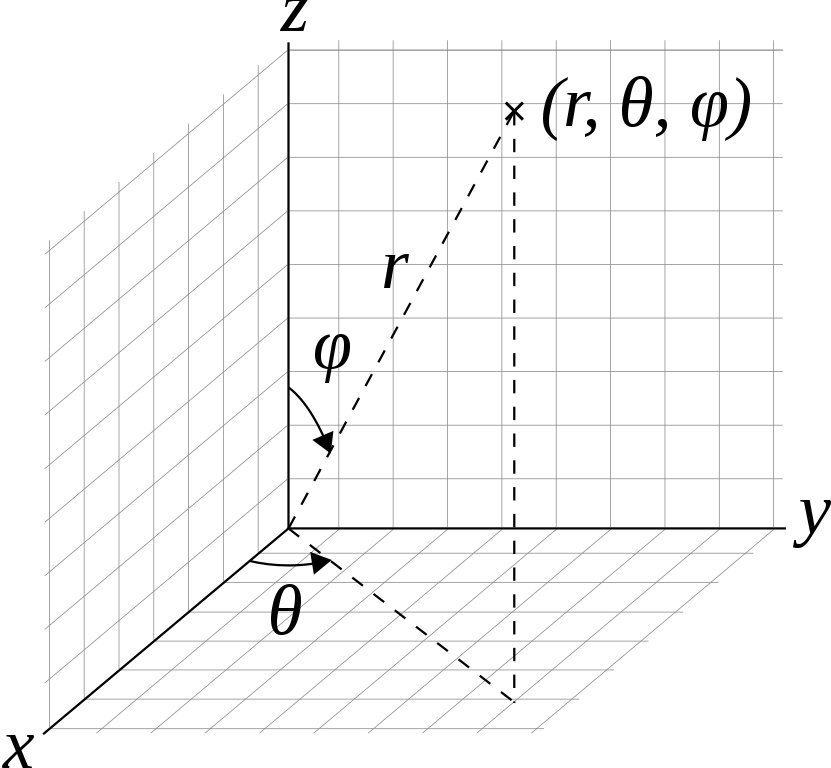
\includegraphics[scale=0.3]{img/831px-3D_Spherical_2.png}
    \caption{Visualisation of the \href{  https://en.wikipedia.org/wiki/Spherical_coordinate_system }{spherical coordinate frame} in relation to the cartesian one.}
    \label{fig:enter-label}
\end{figure}

There is no one single way to find a polynomial transforming one vector into the other. A way to do it involves finding the vector cross product of the 2 vectors - say $v$ and  $u$ - to represent the rotation axis, and their dot product to determine the angle of rotation:
\begin{equation}
    q = v\cdot u + \sqrt{u\bar{u}v\bar{v}} + v \times u
\end{equation}
Applying this method to the 2 vectors in the map given at the beginning we obtain:
\begin{equation}
    q = 1 + \cos{\theta} + \sin{\theta}(\cos{\psi}j-\sin{\psi}i)
\end{equation}
This polynomial does not have unit norm, but does describe the correct rotation.
We can projectivise it by using the half tangent formulas for the trigonometric functions. Since this is all in a projective space, the motion polynomial can be multiplied by any scalar - in this case its norm polynomial - and still produce the same motion.
\begin{equation}
    C(u,t) = 1+u^{2}-2tui - t(u^{2}-1)j
\end{equation}
This is the polynomial who's properties are investigated in the remainder of this report. 
\section{Results}
In order to better visualise the procedure being followed, a network will be used to describe the sequence of transformations from one link to another. This is similar to how voltages are described in an electrical network.
First the overall transformation can be described as such:

\begin{figure}[h!]
\begin{center}
\begin{tikzpicture}[block/.style = {draw, fill=white, rectangle, minimum height=3em, minimum width=3em},
sum/.style= {draw, fill=white, circle, node distance=1cm},
input/.style = {coordinate},
tmp/.style = {coordinate},
output/.style= {coordinate},
pinstyle/.style = {pin edge={to-,thin,black}},
auto,
node distance = 2cm,
>=latex'
]


    \node [block, fill=gray!30] (id) {id};
    \node [block, right of=id, fill=green!30, node distance=4cm] (end) {Goal};

    \draw [->] (id) -- node{$C(u,t)$}(end);

\end{tikzpicture}
\caption{The origin is colored gray, and effector transformation is colored green.}
\label{}
\end{center}
\end{figure}
The transformation between 2 vertices is given by the previously described map \ref{act}(this map also works for quaternions). By factorising, we will obtain an equivalent transformation sequence, which is directly realisable mechanically using elementary joints. This can be symbolically described as follows:

\begin{figure}[h!]
\begin{center}
\begin{tikzpicture}[block/.style = {draw, fill=white, rectangle, minimum height=3em, minimum width=3em, node distance=2.5cm},
sum/.style= {draw, fill=white, circle, node distance=1cm},
input/.style = {coordinate},
tmp/.style = {coordinate},
output/.style= {coordinate},
pinstyle/.style = {pin edge={to-,thin,black}},
auto,
node distance = 2cm,
>=latex'
]


    \node [block, fill=gray!30] (id) {id};
    \node [block,right of=id] (link1) {link1};
    \node [block,right of=link1] (link2) {link1};
    \node [block, right of=link2, fill=green!30, node distance=2.5cm] (end) {Goal};

    \draw [->] (id) -- node{$H_1(u,t)$}(link1);
    \draw [->] (link1) -- node{$H_2(u,t)$}(link2);
    \draw [->] (link2) -- node{$H_3(u,t)$}(end);

    \draw [->] (id) to [out=-90,in=-90] node{$C(u,t)$}(end);

\end{tikzpicture}
\caption{The 2 paths to the goal would describe the same motion by construction}
\label{}
\end{center}
\end{figure}

The factorization methods for multivariate biquaterionic polynomials are still in their infancy\cite{ lercher2021multiplication, Lercher_2022 }. The methods used for the univariate case are more developed, but break down in the multivariate case quite spectacularly, producing factors which change their geometry during movement. However, as this is a very simple case, the factorization can be done by hand manually producing the following factorization:
\begin{equation}
    C(u,t) = (1+uk)(1+jt)(1-uk)
\end{equation}
This factorization is interesting, as it can be thought of as a rotation around the y axis, which is first rotated around the z axis. 
The first problem here is that this is a 3R chain which is supposed to perform a 2DOF motion. For that to be the case the movement has to be constrained. In the univariate case this is done by connecting multiple factorizations of the same movement  to the end effector. If described using a diagram it would look like this:

\begin{figure}[h!]
\begin{center}
\begin{tikzpicture}[block/.style = {draw, fill=white, rectangle, minimum height=3em, minimum width=3em, node distance=2.5cm},
sum/.style= {draw, fill=white, circle, node distance=1cm},
input/.style = {coordinate},
tmp/.style = {coordinate},
output/.style= {coordinate},
pinstyle/.style = {pin edge={to-,thin,black}},
auto,
node distance = 2cm,
>=latex'
]


    \node [block, fill=gray!30] (id) {id};
    \node [block,below right of=id] (link1) {link 1};
    \node [block,right of=link1] (link2) {link 2};
    \node [block,above right of=id] (link3) {link 3};
    \node [block,right of=link3] (link4) {link 4};
    \node [block, above right of=link2, fill=green!30, node distance=2.5cm] (end) {Goal};

    \draw [->] (id) -- node{$H_1(u,t)$}(link1);
    \draw [->] (link1) -- node{$H_2(u,t)$}(link2);
    \draw [->] (link2) -- node{$H_3(u,t)$}(end);

    \draw [->] (id) -- node{$G_1(u,t)$}(link3);
    \draw [->] (link3) -- node{$G_2(u,t)$}(link4);
    \draw [->] (link4) -- node{$G_3(u,t)$}(end);

    \draw [->] (id) -- node{$C(u,t)$}(end);

\end{tikzpicture}
\caption{A hypothetical alternate factorization}
\label{}
\end{center}
\end{figure}



Here however that is impossible, as it was found that no other factorization exists. Not to mention, even if it were possible, another constraint would have to be imposed on the mechanism in the form of another loop. This is because according to the mobility formula for spherical mechanisms:
\begin{equation}
    M = J - 3L
\end{equation}
Where J is the number of joints of the mechanism, and L the number of independent loop closure conditions, the mobility of such mechanism would be 3, not 2. Usually these kinds of parallel mechanisms have 3 joints in one arm, and 2 in the other. This way only one loop is needed. It is unclear at the moment how such a factorization could be created, but it would necessitate a different form of the factor representing elementary motions. \\
Another approach was tried, where an artificial scaffolding would be constructed around the main mechanism, which would create the necessary constraints. There are 2 possible topologies for such a scaffold:
\begin{figure}[h!]
\begin{center}
\begin{tikzpicture}[block/.style = {draw, fill=white, rectangle, minimum height=3em, minimum width=3em, node distance=3cm},
sum/.style= {draw, fill=white, circle, node distance=1cm},
input/.style = {coordinate},
tmp/.style = {coordinate},
output/.style= {coordinate},
pinstyle/.style = {pin edge={to-,thin,black}},
auto,
node distance = 2cm,
>=latex'
]


    \node [block, fill=gray!30] (id) {id};
    \node [block,right of=id] (link1) {link1};
    \node [block,right of=link1] (link2) {link2};
    \node [block, right of=link2, fill=green!30, node distance=3cm] (end) {Goal};

    \node [block, above of=id] (ids) {scaf 1};
    \node [block,right of=ids] (link1s) {scaf 2};
    \node [block,right of=link1s] (link2s) {scaf 3};
    \node [block, right of=link2s, node distance=3cm] (ends) {scaf 4};




    \draw [->] (id) -- node{$P_1(u,t)$}(ids);
    \draw [->] (link2) -- node{$P_2(u,t)$}(link2s);
    \draw [->] (end) -- node{$P_3(u,t)$}(ends);

    \draw [->] (id) -- node{$H_1 = 1+uk$}(link1);
    \draw [->] (link1) -- node{$H_2 = 1+jt$}(link2);
    \draw [->] (link2) -- node{$H_3 = 1-uk$}(end);

    \draw [->] (ids) -- node{$G_1(u,t)$}(link1s);
    \draw [->] (link1s) -- node{$G_2(u,t)$}(link2s);
    \draw [->] (link2s) -- node{$G_3(u,t)$}(ends);

    \draw [->] (id) to [out=-90,in=-90] node{$C(u,t)$}(end);

\end{tikzpicture}
\begin{tikzpicture}[block/.style = {draw, fill=white, rectangle, minimum height=3em, minimum width=3em, node distance=3cm},
sum/.style= {draw, fill=white, circle, node distance=1cm},
input/.style = {coordinate},
tmp/.style = {coordinate},
output/.style= {coordinate},
pinstyle/.style = {pin edge={to-,thin,black}},
auto,
node distance = 2cm,
>=latex'
]


    \node [block, fill=gray!30] (id) {id};
    \node [block,right of=id] (link1) {link1};
    \node [block,right of=link1] (link2) {link2};
    \node [block, right of=link2, fill=green!30, node distance=3cm] (end) {Goal};

    \node [block, above of=id] (ids) {scaf 1};
    \node [block,right of=ids] (link1s) {scaf 2};
    \node [block,right of=link1s] (link2s) {scaf 3};
    \node [block, right of=link2s, node distance=3cm] (ends) {scaf 4};




    \draw [->] (id) -- node{$P_1(u,t)$}(ids);
    \draw [->] (link1) -- node{$P_2(u,t)$}(link1s);
    \draw [->] (end) -- node{$P_3(u,t)$}(ends);

    \draw [->] (id) -- node{$H_1 = 1+uk$}(link1);
    \draw [->] (link1) -- node{$H_2 = 1+jt$}(link2);
    \draw [->] (link2) -- node{$H_3 = 1-uk$}(end);

    \draw [->] (ids) -- node{$G_1(u,t)$}(link1s);
    \draw [->] (link1s) -- node{$G_2(u,t)$}(link2s);
    \draw [->] (link2s) -- node{$G_3(u,t)$}(ends);

    \draw [->] (id) to [out=-90,in=-90] node{$C(u,t)$}(end);

\end{tikzpicture}
\caption{Second scaffold creates a 4 bar near the base of the mechanism, whle the first near the end}
\label{}
\end{center}
\end{figure}

\clearpage
The polynomial $P_2$ can be more or less chosen arbitrarily. It was chosen however, to make the 4 bars univariate. In each of these topologies, there are 3 ways to choose the factors, giving 6 cases to consider. Regrettably, none of these cases produced a viable mechanism. 
\\
Finally, to determine where it all went wrong, an attempt was made to analyse an actual 2DOF spherical manipulator using this method. The manipulator chosen was a simplified version of the 3DOF "Agile Eye" manipulator developed by dr. Gosselin . 
A system of equations was developed based on the description of how the passive joint angles depend on the 2 active ones. It was found that its solution was impossibly complicated, included multiple nested square roots, and was in a singular configuration at the origin. This could have several explanations, the most probable of which is that the assumption of 2 factorizations, one having 3 linear factors, the other 2, was wrong. It remains to be seen what would be the appropriate way to describe such a system with quaterionic polynomials.

\section{Discussion}
On the surface the project can be deemed a failure. The goal of creating a manipulator using polynomial factorization was not met. However where the 
issues with this method lie was greatly elucidated. Decomposition into
linear factors is something that mathematicians are interested in, but 
for the purpose of manipulator design, it may be more worthwhile to look
into factorizations int o factors producing linear, or rotational motion. 
For example, one way to represent a translation using a biquaterionic polynomial is:
\begin{equation}
    H(y) = 1 - \varepsilon t v
\end{equation}
However, another way to do it is with a quadratic polynomial:
\begin{equation}
    H(t) = 1 +t^2 + t^{2} \varepsilon v
\end{equation}
This is still a linear motion, but bounded instead of unbounded. 
Similar alternative representations can be found for rotational motion.
Future investigations should attempt to use these alternative representations in the multivariate case to construct viable mechanisms.
